\section{Experimente}

\begin{frame}
    \frametitle{Stärkere Gewichtung des $ L_{style} $}

    \begin{figure}[H]
        \centering
        \begin{subfigure}[h]{0.49\textwidth}
            \centering
            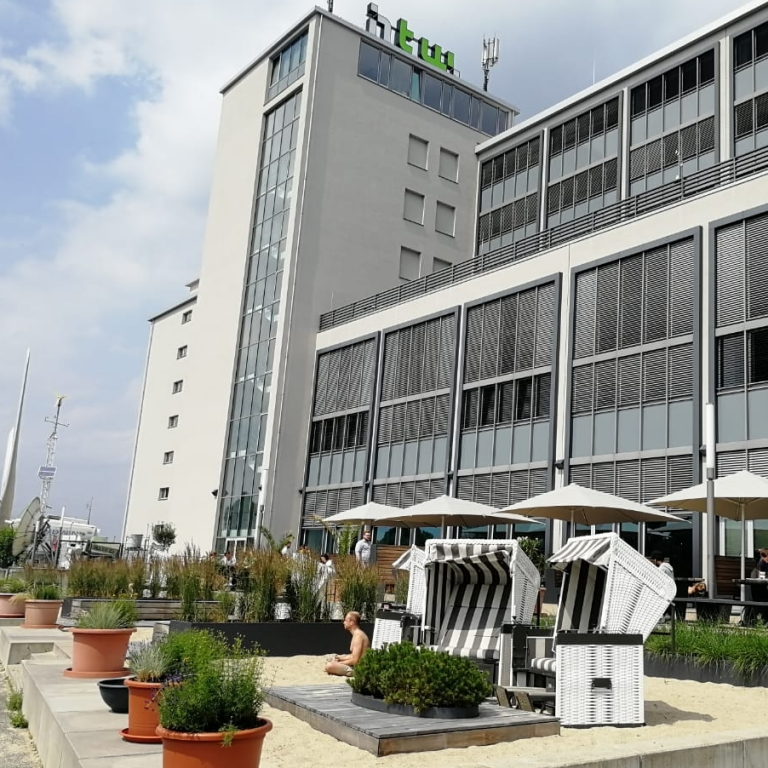
\includegraphics[width=\textwidth]{resources/content/content/htw-768x768.jpg}
        \end{subfigure}
        \begin{subfigure}[h]{0.49\textwidth}
            \centering
            \includegraphics[width=\textwidth]{resources/content/style/the_scream.jpg}
        \end{subfigure}
        \caption{HTW kombiniert mit \textit{The Scream} \cite{the_scream_img}}
    \end{figure}
\end{frame}

\begin{frame}
    \frametitle{Stärkere Gewichtung des $ L_{style} $}

    \begin{figure}[H]
        \centering
        \begin{subfigure}[h]{0.49\textwidth}
            \centering
            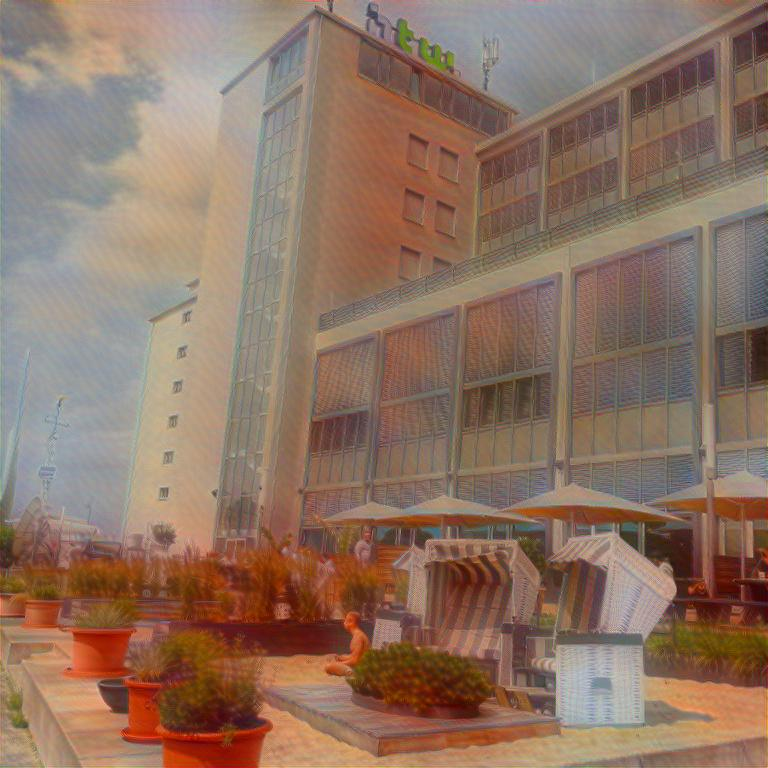
\includegraphics[width=\textwidth]{resources/content/experiments/a__the_scream__768x768__style-weight_1e+06__tv-weight_0e+00.jpg}
        \end{subfigure}
        \begin{subfigure}[h]{0.49\textwidth}
            \centering
            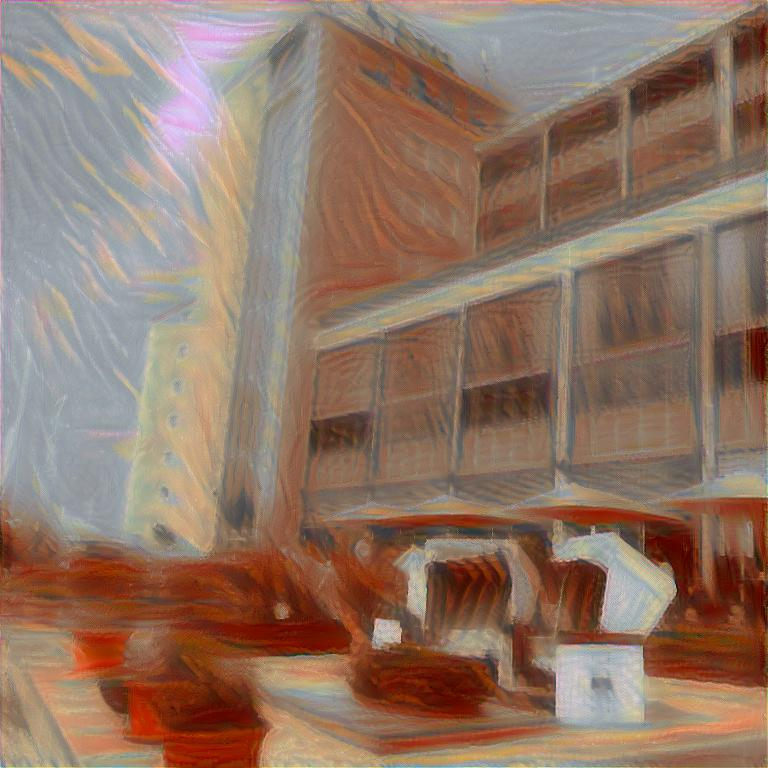
\includegraphics[width=\textwidth]{resources/content/experiments/a__the_scream__768x768__style-weight_1e+09__tv-weight_0e+00.jpg}
        \end{subfigure}
        \caption{\textit{The Scream} mit $ \alpha = 1 $, $ \beta = 10^{6} $ und $ \beta = 10^{9} $, $ \gamma = 0 $}
    \end{figure}
\end{frame}


\begin{frame}
    \frametitle{Verwendete Netzwerkarchitekturen}

    \begin{table}[H]
        \centering
        \begin{tabular}{ |c|c|c|c| }
            \hline
            \textbf{Name} & \textbf{Bottleneck Size $ s $} & \textbf{Multiplikator $ m $} & \textbf{Parameter} \\ \hline
            Netzwerk 1 & 5 & 32 & 2.007.881     \\ \hline
            Netzwerk 2 & 5 & 16 & 507.305       \\ \hline
            Netzwerk 3 & 5 & 8  & 129.497       \\ \hline
            Netzwerk 4 & 5 & 4  & 33.713        \\ \hline
    
            Netzwerk 5 & 4 & 32 & 1.712.073     \\ \hline
            Netzwerk 6 & 4 & 16 & 433.129       \\ \hline
            Netzwerk 7 & 4 & 8  & 110.841       \\ \hline
            Netzwerk 8 & 4 & 4  & 28.993        \\ \hline
        \end{tabular}
        \caption{Unterschiedliche Netzwerkgrößen und ihre Parameter}
        \label{tab:networks}
    \end{table}
\end{frame}


\begin{frame}
    \frametitle{Verwendete Netzwerkarchitekturen}

    \begin{table}[H]
        \centering
        \begin{tabular}{ |c|c|c|c| }
            \hline
            \textbf{Name} & \textbf{Bottleneck Size $ s $} & \textbf{Multiplikator $ m $} & \textbf{Parameter} \\ \hline
            Netzwerk 9  & 3 & 32 & 1.416.265    \\ \hline
            Netzwerk 10 & 3 & 16 & 358.953      \\ \hline
            Netzwerk 11 & 3 & 8  & 92.185       \\ \hline
            Netzwerk 12 & 3 & 4  & 24.273       \\ \hline
    
            Netzwerk 13 & 2 & 32 & 1.120.457    \\ \hline
            Netzwerk 14 & 2 & 16 & 284.777      \\ \hline
            Netzwerk 15 & 2 & 8  & 73.529       \\ \hline
            Netzwerk 16 & 2 & 4  & 19.553       \\ \hline
        \end{tabular}
        \caption{Unterschiedliche Netzwerkgrößen und ihre Parameter}
        \label{tab:networks}
    \end{table}
\end{frame}


 \begin{frame}
     \frametitle{Verwendete Geräte}
 
     
     \begin{itemize}
         \item Dell XPS 15 9550
         \item Jetson TX2
     \end{itemize}
 \end{frame}


 \begin{frame}
     \frametitle{Performanz-Test mit 1920 * 1080 (Full HD) Pixel Bildern}
 
    \begin{table}[H]
        \centering
        \begin{tabular}{ |c|c|c|c|c| }
            \hline
            \textbf{Name} & \textbf{XPS - GPU} & \textbf{Jetson - GPU}   \\ \hline
            Network  1 & \textcolor{danger}{nicht durchführbar} & \textcolor{danger}{nicht durchführbar} \\ \hline
            Network  2 & \textcolor{danger}{nicht durchführbar} & 0,86413                                \\ \hline
            Network  3 & \textcolor{danger}{nicht durchführbar} & 0,48424                                \\ \hline
            Network  4 & \textcolor{danger}{nicht durchführbar} & 0,35886                                \\ \hline
            Network  5 & \textcolor{danger}{nicht durchführbar} & \textcolor{danger}{nicht durchführbar} \\ \hline
            Network  6 & \textcolor{danger}{nicht durchführbar} & 0,70640                                \\ \hline
            Network  7 & \textcolor{danger}{nicht durchführbar} & 0,39689                                \\ \hline
            Network  8 & \textcolor{danger}{nicht durchführbar} & 0,30227                                \\ \hline
        \end{tabular}
        \caption{Berechnungsgeschwindigkeit in Sekunden für Bilder der Größe 1920 * 1080 Pixel}
        \label{tab:1920x1080}
    \end{table}
    
 \end{frame}

 \begin{frame}
    \frametitle{Performanz-Test mit 1920 * 1080 (Full HD) Pixel Bildern}

   \begin{table}[H]
       \centering
       \begin{tabular}{ |c|c|c|c|c| }
           \hline
           \textbf{Name} & \textbf{XPS - GPU} & \textbf{Jetson - GPU}   \\ \hline
           Network  9 & \textcolor{danger}{nicht durchführbar} & 0,67149                                \\ \hline
           Network 10 & \textcolor{danger}{nicht durchführbar} & 0,51339                                \\ \hline
           Network 11 & \textcolor{danger}{nicht durchführbar} & 0,30213                                \\ \hline
           Network 12 & \textcolor{danger}{nicht durchführbar} & 0,24884                                \\ \hline
           Network 13 & \textcolor{danger}{nicht durchführbar} & 0,37438                                \\ \hline
           Network 14 & \textcolor{danger}{nicht durchführbar} & 0,25658                                \\ \hline
           Network 15 & \textcolor{danger}{nicht durchführbar} & 0,21752                                \\ \hline
           Network 16 & 0,00454                                & 0,19545                                \\ \hline
       \end{tabular}
       \caption{Berechnungsgeschwindigkeit in Sekunden für Bilder der Größe 1920 * 1080 Pixel}
       \label{tab:1920x1080}
   \end{table}
\end{frame}

\begin{frame}
    \frametitle{Loss: The Scream}

    \begin{figure}[H]
        \centering
        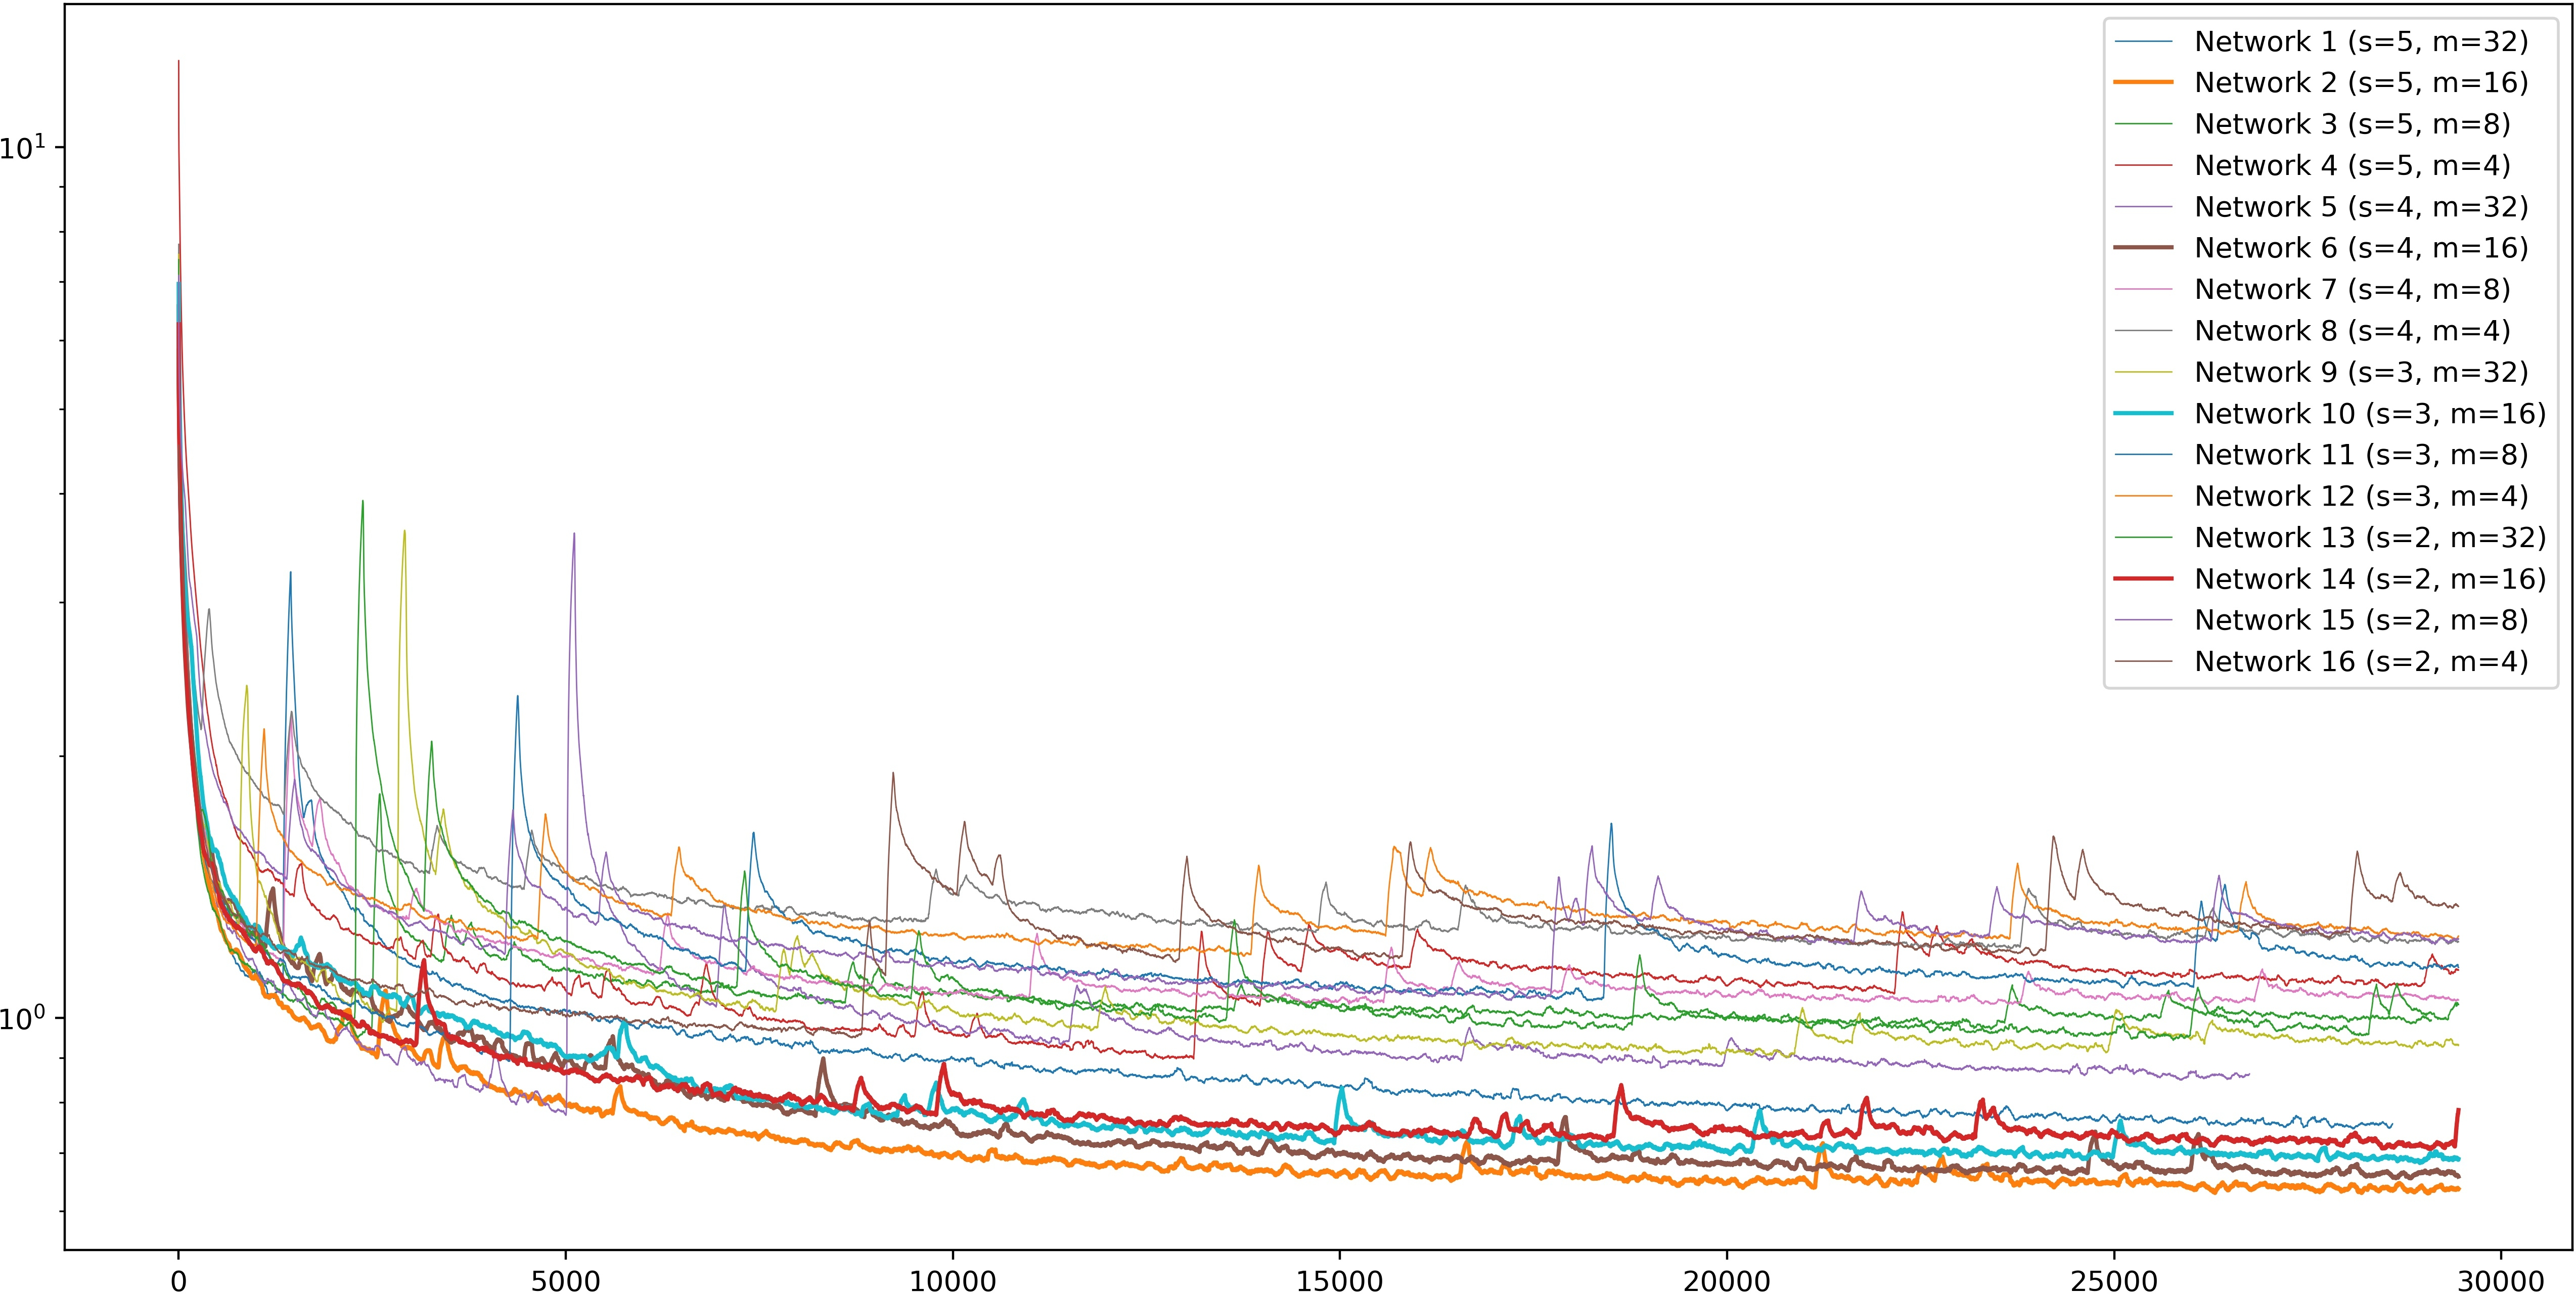
\includegraphics[width=1.00\textwidth]{resources/content/experiments/fast_loss_plot_experiment2.jpg}
        \caption{Loss: The Scream}
        \label{img:results_the_scream}
    \end{figure}    
\end{frame}